\documentclass{beamer}

\usepackage[english, russian]{babel}
\usepackage{minted}
\usepackage[T1]{fontenc}
\usepackage[utf8]{inputenc}
\usepackage{amsmath}

\title{Генерация случайных чисел}
\author{Карасев Арсений Михайлович}
\date{2021г.}
\usetheme{Warsaw}
\institute{{Саратовский национальный исследовательский государственный университет} \\
    им.~Н.~Г.~Чернышевского \\[5pt]
Кафедра математической кибернетики\\ и компьютерных наук\\[5pt]
Научный руководитель: доцент Иванова ~А.~С.
}

\begin{document}
% \renewcommand\theFancyVerbLine{\small\arabic{FancyVerbLine}}

\begin{frame}
\titlepage
\end{frame}


\begin{frame}
\frametitle{Виды случайных чисел}
\begin{columns}[t]
\begin{column}{0.5\textwidth}
Истинные случайные числа.
\begin{itemize}
\item
Основываются на непредсказуемых данных физических явлений, например анализ шумов в звуковой карте компьютера.
\end{itemize}
\end{column}
\begin{column}{0.5\textwidth}
Псевдослучайные числа.
\begin{itemize}
\item
Основываются на определённых математических алгоритмах. За основу берётся какое--то стартовое число. Каждое новое число в последовательности ГПСЧ генерируется исходя из предыдущего определенным способом.
\end{itemize}
\end{column}
\end{columns}
\end{frame}


\begin{frame}[fragile]
\frametitle{Пример простого ГПСЧ (Генератора псевдослучайных чисел)}
\begin{minted}[mathescape, linenos, numbersep=5pt, frame=lines, framesep=2mm]{cpp}
int PRNG()
{
	static unsigned long int seed = 5643;
	seed = seed * 1103515245 + 12345;
	return (unsigned int)(seed / 65536) % 32768;
}
\end{minted}
Сама <<случайность>> происходит из--за переполнения, так как в математических операциях участвуют довольно большие числа.
\end{frame}


\begin{frame}
\frametitle{Распределения. Ключевые термины}
\begin{itemize}
\item<1->
Распределение вероятностей --- это закон, описывающий область значений случайной величины и соответствующие вероятности появления этих значений. 
\item<2->
Плотность вероятности --- вещественная функция, характеризующая сравнительную вероятность реализации тех или иных значений случайной переменной. 
\item<3->
Функция распределения в теории вероятностей --- функция, характеризующая распределение случайной величины.
\item<4->
Математическое ожидание ($\mu$) --- среднее значение случайной величины. В случае непрерывной случайной величины подразумевается взвешивание по плотности распределения.
\item<5->
Среднеквадратическое отклонение ($\sigma$) --- наиболее распространённый показатель рассеивания значений случайной величины относительно её математического ожидания.
\end{itemize}
\end{frame}


\begin{frame}
\frametitle{Равномерное распределение}
\begin{columns}[T,onlytextwidth]
\begin{column}{0.4\textwidth}
\begin{itemize}
\item
Одинаковая вероятность появления для всех чисел в диапазоне.
\item
Идеальное распределение для ГПСЧ.
\end{itemize}
\end{column}
\begin{column}{0.6\textwidth}
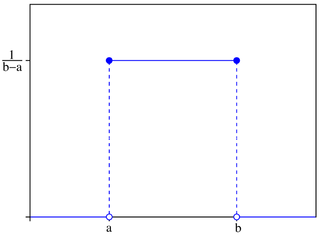
\includegraphics[width=\textwidth]{aVhsm.png}
\end{column}
\end{columns}
\end{frame}


\begin{frame}
\frametitle{Гауссово распределение (Нормальное)}
\begin{columns}[T,onlytextwidth]
\begin{column}{0.5\textwidth}
\small
\begin{itemize}
\item
Стандартным нормальным распределением называется нормальное распределение с математическим ожиданием $\mu = 0$ и стандартным отклонением $\sigma = 1$
\item
Нормальное распределение --- распределение вероятностей, которое в одномерном случае задаётся функцией плотности вероятности, совпадающей с функцией Гаусса:
$ f(x)={\frac {1}{\sigma {\sqrt {2\pi }}}}\;\exp {\biggl (}{-{\frac {(x-\mu )^{2}}{2\sigma ^{2}}}}{\biggr )} $
\end{itemize}
\end{column}
\begin{column}{0.5\textwidth}
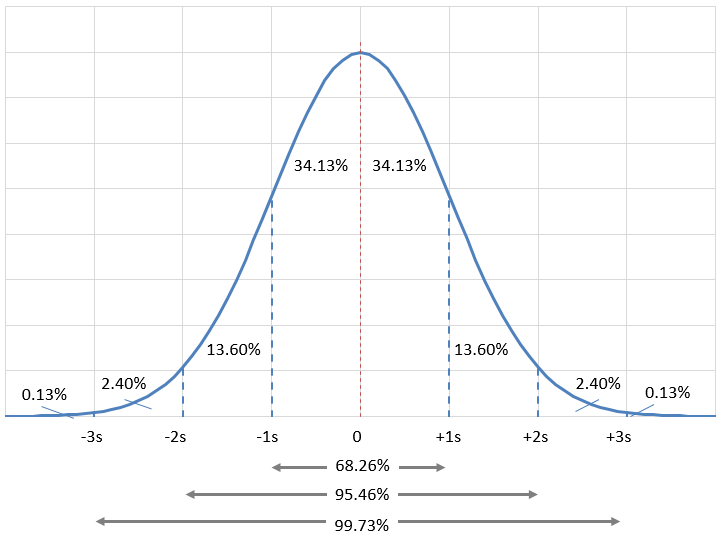
\includegraphics[width=\textwidth]{20-5-Normal-distribution.png}
\end{column}
\end{columns}
\end{frame}


\begin{frame}[fragile]
\frametitle{Код реализации генерации случайных чисел на нормальном распределении}
\tiny
\begin{minted}[mathescape, linenos, numbersep=5pt, frame=lines, framesep=2mm]{cpp}
double normalFunction(double x)
{
    if (x == 0.5) {
        return 0.0;
    }
    if (x < eps) {
        return -4.3;
    }
    if (x > 1 - eps) {
        return 4.3;
    }


    int sign = 1;
    if (x < 0.5) {
        x = 1 - x;
        sign = -1;
    }
    double xk1 = values[(int)(round(10 * x) - 5)], xk = xk1;
    double b = 1 - 2 * x;
    do 
    {
        xk = xk1;
        double t = xk / sqrt_2;
        xk1 = xk - sqrt_pi_2 * exp(t * t) * (erf(t) + b);
    } 
    while (fabs(xk - xk1) >= eps);

    return sign == 1 ? xk1 : -xk1;
}
\end{minted}
\end{frame}


\begin{frame}[fragile]
\frametitle{Код реализации генерации случайных чисел на нормальном распределении}
\scriptsize
\begin{minted}[mathescape, linenos, numbersep=5pt, frame=lines, framesep=2mm]{cpp}
double getNormRandVal()
{
    return normalFunction((double)rand() / ((double)RAND_MAX));
}


double finalResult(double m, double sigma)
{
    std::vector<double> vec;
    double randNum;
    randNum = m + sigma * getNormRandVal();


    return randNum;
}
\end{minted}
Где values --- массив с вычисленными значениями функции нормального распределения (от 0.5 до 0.99)
\end{frame}


\begin{frame}
\frametitle{Результат работы генератора}
\begin{columns}[T]
\begin{column}{0.35\textwidth}
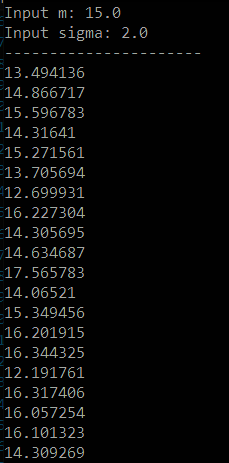
\includegraphics[width=\textwidth]{res_norm_dist1.png}
\end{column}
\begin{column}{0.45\textwidth}
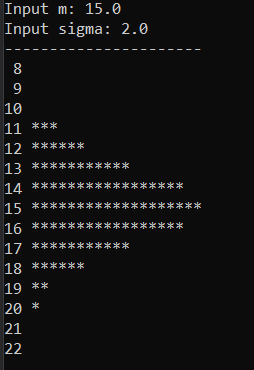
\includegraphics[width=\textwidth]{res_norm_dist2.png}
\end{column}
\end{columns}
\end{frame}


\begin{frame}
\Large
\begin{columns}[T]
\begin{column}{0.5\textwidth}
Получается, мы <<переводим>> равномерное распределение в нормальное.
\end{column}
\begin{column}{0.6\textwidth}
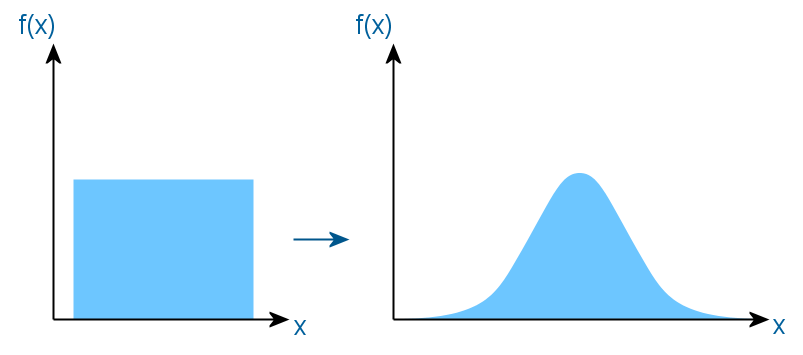
\includegraphics[width=\textwidth]{31764eb4365ae9ea42cbdd270b6e6513.png}
\end{column}
\end{columns}
\end{frame}


\begin{frame}
\frametitle{Экспоненциальное распределение (показательное)}
\begin{columns}[T]
\begin{column}{0.6\textwidth}
Экспоненциальное распределение моделирует время между двумя последовательными свершениями одного и того же события.
Для подсчёта вероятности нужен один параметр ($\lambda$), причём $\lambda > 0$. Тогда плотность вероятности этого распределения
имеет вид:

\begin{equation*}
f_{X}(x) = 
 \begin{cases}
   \lambda\,e^{{-\lambda x}}, x\ge 0, \\
   0, x<0.
 \end{cases}
\end{equation*}
\end{column}
\begin{column}{0.5\textwidth}
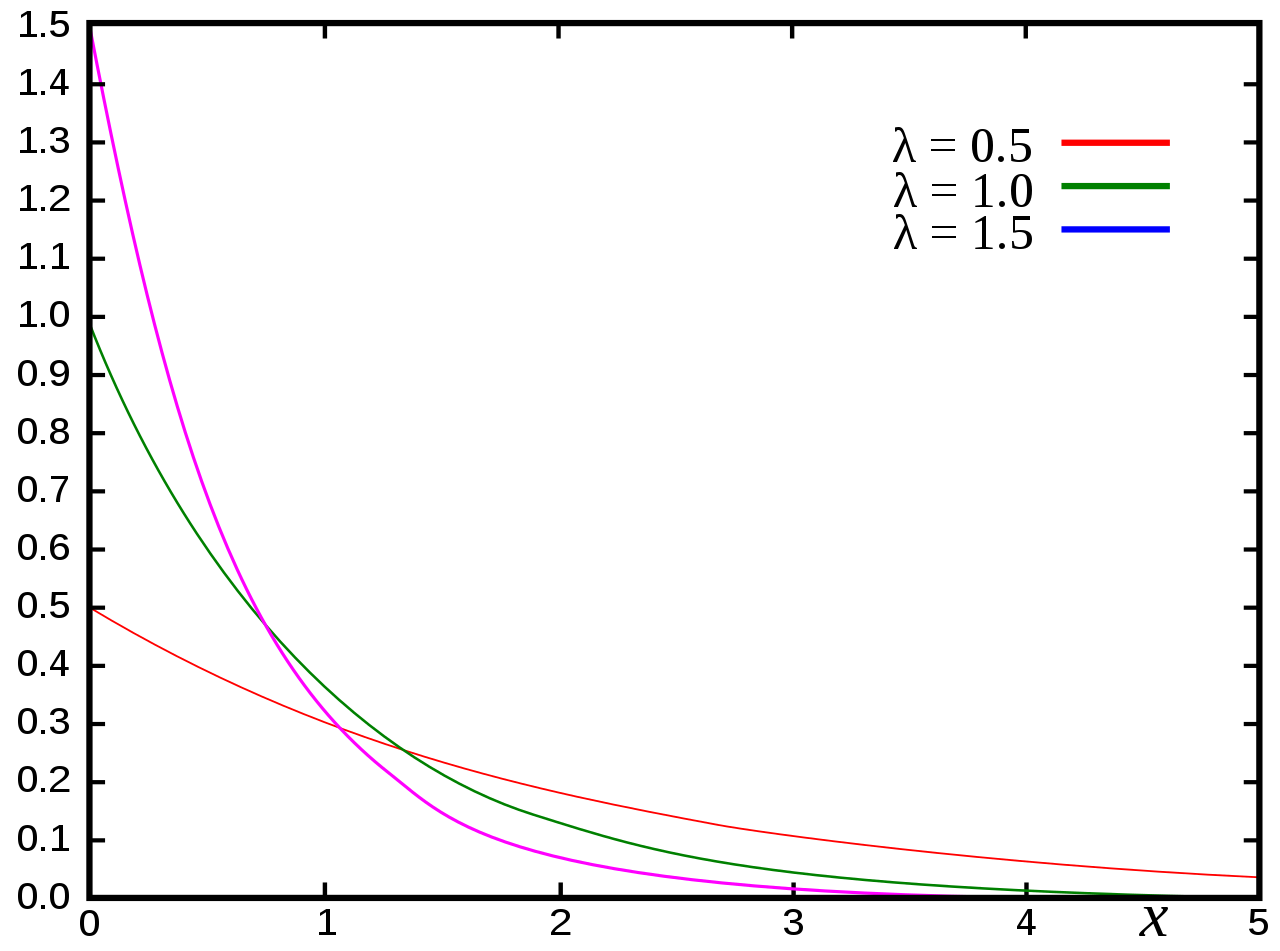
\includegraphics[width=\textwidth]{1280px-Exponential_distribution_pdf.svg.png}
\end{column}
\end{columns}
\end{frame}


\begin{frame}[fragile]
\frametitle{Код реализации генератора случайных чисел на экспоненциальном распределении}
\begin{minted}[mathescape, linenos, numbersep=5pt, frame=lines, framesep=2mm]{cpp}
double getRandomnumber()
{
	return (double)rand() / (double)RAND_MAX;
}


double exponentialDistribution(double ly)
{
	double x, u;
	u = getRandomnumber();
	x = log(1 - u) * (1 / (-ly));
	return x;
}
\end{minted}
\end{frame}


\begin{frame}
\frametitle{Результат работы генератора}
\begin{columns}[t]
\begin{column}{0.25\textwidth}
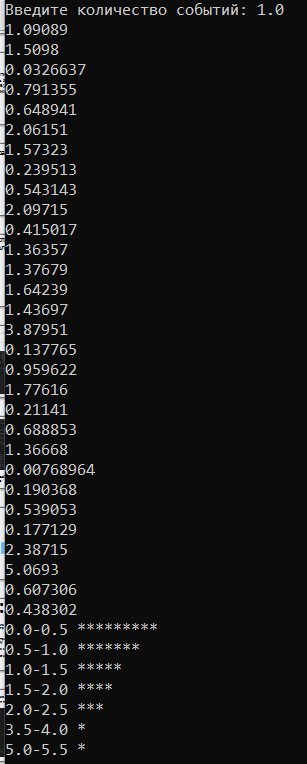
\includegraphics[width=\textwidth]{exp_dist1.png}
\end{column}
\begin{column}{0.25\textwidth}
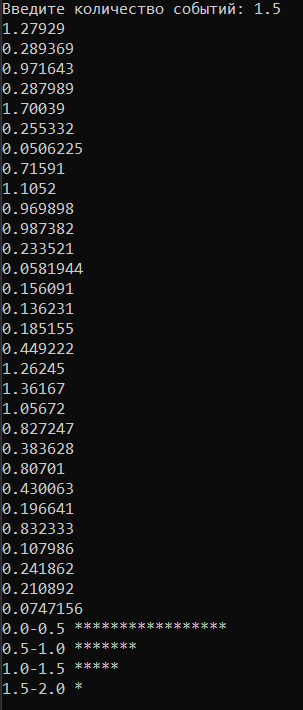
\includegraphics[width=\textwidth]{exp_dist2.png}
\end{column}
\begin{column}{0.25\textwidth}
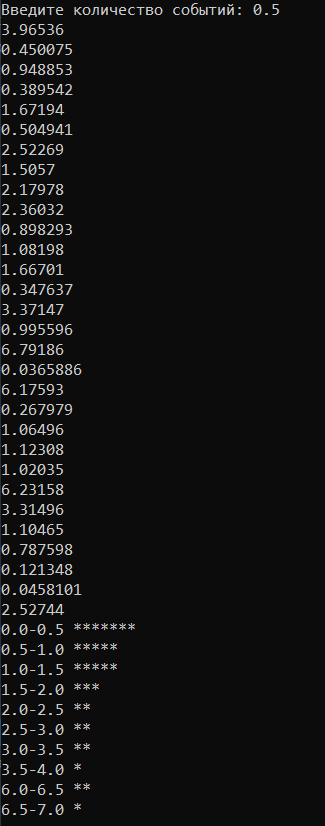
\includegraphics[width=\textwidth]{exp_dist3.png}
\end{column}
\end{columns}
\end{frame}


\begin{frame}[t]
\frametitle{Список использованной литературы}
\tiny
\begin{thebibliography}{9}
\setbeamertemplate{bibliography item}[article]

\bibitem{Gnedenko2019}
{Б. В. Гнеденко}
\newblock {Курс теории вероятностей}~/Б. В. Гнеденко.
\newblock Москва, Россия, Едиториал УРСС, 2019, стр. 158--175.

\bibitem{Chistyakov1987}
{В.П. Чистяков}
\newblock {Курс теории вероятностей}~/Б. В. Гнеденко.
\newblock Москва, Россия, Наука, 1987, стр. 71--122.

\setbeamertemplate{bibliography item}[online]

\bibitem{trueRandGen}
{Поиск генераторов истинных случайных чисел[Электронный ресурс]}
\newblock URL: https://habr.com/ru/company/mailru/blog/408181/
\newblock (Дата обращения 13.11.2017) Загл. с экр. яз. рус.

\bibitem{randNumGen}
{Генерация случайных чисел[Электронный ресурс]}
\newblock URL: https://ravesli.com/urok-71-generatsiya-sluchajnyh-chisel-funktsii-srand-i-rand/
\newblock (Дата обращения 15.09.2020) Загл. с экр. яз. рус.

\bibitem{randNumGenDist}
{Генераторы непрерывно распределенных случайных величин[Электронный ресурс]}
\newblock URL: URL: https://habr.com/ru/post/263993/
\newblock (Дата обращения 02.08.2015) Загл. с экр. яз. рус.
\end{thebibliography}
\end{frame}


\begin{frame}
\huge
\begin{center}
Спасибо за внимание!
\end{center}
\end{frame}

\end{document}